\section{More on STL}

\begin{frame}{6 Components}
    \begin{itemize}
        \item Containers
        \begin{itemize}
            \item \blue{Sequential containers}: \ttt{list}, \ttt{vector}, \ttt{deque}, \dots
            \item Associative containers
            \begin{itemize}
                \item Ordered: \ttt{map}, \ttt{set}, \ttt{multimap}, \ttt{multiset} \textbf{(RB-tree)}
                \item Unordered: \ttt{unordered\_map}, \ttt{unordered\_set}, \ttt{unordered\_multimap}, \ttt{unordered\_multiset} \textbf{(Hash-table)}
            \end{itemize}
        \end{itemize}
        \item \blue{Iterators}
        \item \blue{Algorithms}
        \item Adapters
        \begin{itemize}
            \item Container adapters: \ttt{stack}, \ttt{queue}, \ttt{priority\_queue}
            \item Iterator adapters: Insert iterators, stream iterators, reverse iterators, move iterators
        \end{itemize}
        \item Allocators
        \item Functors
        \begin{itemize}
            \item \ttt{std::plus}, \ttt{std::minus}, \ttt{std::less}, \dots
            \item \ttt{std::function}, \ttt{std::bind}, \dots
        \end{itemize}
    \end{itemize}
\end{frame}

\subsection{Associative Containers}

\begin{frame}[fragile]{Sets}
    Maintain a set of integers. Duplicates should be dropped.
    \begin{cpp}
std::vector<int> v;
int x;
while (std::cin >> x) {
  bool found = false;
  for (auto y : v)
    if (y == x) {
      found = true;
      break;
    }
  if (!found)
    v.push_back(x);
}
    \end{cpp}
\end{frame}

\begin{frame}[fragile]{Sets}
    Use \ttt{std::find}:
    \begin{cpp}
while (std::cin >> x) {
  auto found = std::find(v.begin(), v.end(), x);
  if (found == v.end())
    v.push_back(x);
}
    \end{cpp}
    Still inefficient...
    \pause
    \begin{cpp}
std::set<int> s;
int x;
while (std::cin >> x)
  s.insert(x);
    \end{cpp}
\end{frame}

\begin{frame}[fragile]{Maps}
    Map student numbers to scores:
    \begin{cpp}
int scores[N];
scores[3] = 90;
    \end{cpp}
    Map student names to scores?
    \pause
    \begin{cpp}
std::map<std::string, int> scores;
scores["Alice"] = 90;
    \end{cpp}
\end{frame}

\subsection{Iterator Adapters}

\begin{frame}[fragile]{Insert Iterators}
    Copy elements from a \ttt{vector} to another:
    \begin{cpp}
std::copy(v.begin(), v.end(), v2.begin());
    \end{cpp}
    \textbf{But this requires \ttt{v2} to have enough room.}
    \pause
    \begin{cpp}
v2.resize(v.size());
std::copy(v.begin(), v.end(), v2.begin());
    \end{cpp}
    \pause
    Copy elmeents \textbf{to the end} of another \ttt{vector}?
    \pause
    \begin{cpp}
std::copy(v.begin(), v.end(), std::back_inserter(v2));
    \end{cpp}
\end{frame}

\begin{frame}[fragile]{Stream Iterators}
    Write elements to the output stream?
    \begin{cpp}
std::ostream_iterator<int> out_iter(std::cout, " ");
std::copy(v.begin(), v.end(), out_iter);
    \end{cpp}
    \pause
    Construct a \ttt{vector} from input:
    \begin{cpp}
std::istream_iterator<int> in_iter(std::cin), eof;
std::vector<int> vec(in_iter, eof);
    \end{cpp}
    Use \ttt{back\_inserter} together:
    \begin{cpp}
std::copy(in_iter, eof, std::back_inserter(vec));
    \end{cpp}
\end{frame}

\begin{frame}[fragile]{Stream Iterators}
    \begin{itemize}
        \item \ttt{std::istream\_iterator} is of the category \blue{input-iterator}.
        \item \ttt{std::ostream\_iterator} is of the category \blue{output-iterator}.
    \end{itemize}
    Difference between \blue{forward-iterator}s and \blue{input-iterator}s?\par
    \pause
    \blue{Input-iterator}s are disposable, while \blue{forward-iterator}s provide \textit{multi-pass guarantee}.
    \begin{cpp}
auto tmp = iter;
auto value = *iter;
++tmp;
// *iter == value ?
    \end{cpp}
\end{frame}

\subsection{Special Algorithms}

\begin{frame}[fragile]{Sort}
    Using \ttt{std::sort} on \ttt{std::list} is not allowed...
    \begin{itemize}
        \item \ttt{std::sort} requires \blue{random-access-iterator}s, while \ttt{std::list} provides \blue{bidirectional-iterator}s.
        \item \ttt{std::sort} uses \textbf{Intro-sort}, which is a combination of \textbf{Quick-sort}, \textbf{Heap-sort} and \textbf{Insertion-sort}.
    \end{itemize}
    \pause
    Use \ttt{std::list::sort} instead!
    \begin{cpp}
std::list<int> l = some_value();
l.sort();
    \end{cpp}
    \begin{itemize}
        \item Value type is not required to be \blue{swappable}.
        \item Stable sort.
    \end{itemize}
\end{frame}

\begin{frame}[fragile]{Special Operations for Linked-lists}
    See \textit{C++ Primer} Chapter 10.6.
    \begin{center}
        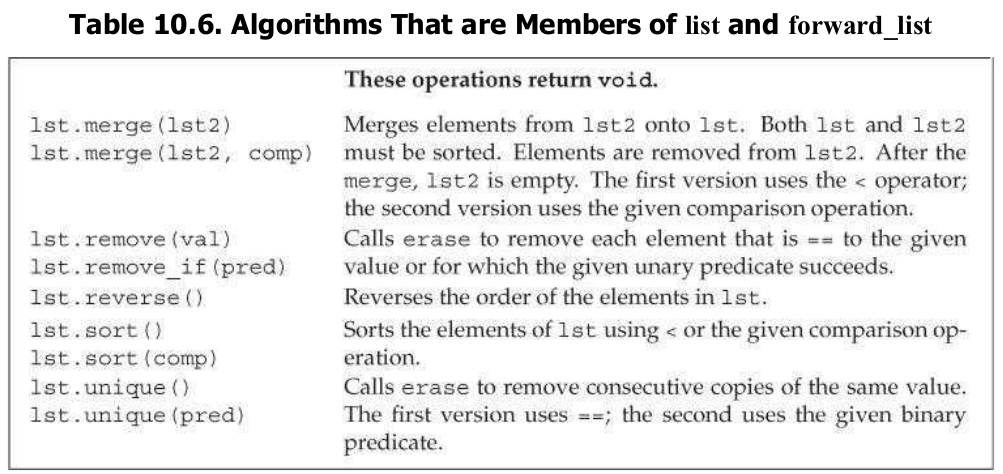
\includegraphics[width=\textwidth]{figures/list_operations.png}
    \end{center}
\end{frame}

\subsection{Allocators}

\begin{frame}{Allocators}
    Consider implementing a \ttt{vector}...
    \begin{itemize}
        \item Separate memory allocation/deallocation and object construction/destruction.
        \item Adopt possibly different methods of memory allocation?
    \end{itemize}
    \pause
    Use different kinds of \blue{allocators} that provide the same interfaces.
\end{frame}

\begin{frame}[fragile]{\ttt{std::allocator}}
    See \textit{C++ Primer} Chapter 12.2.2.
    \begin{center}
        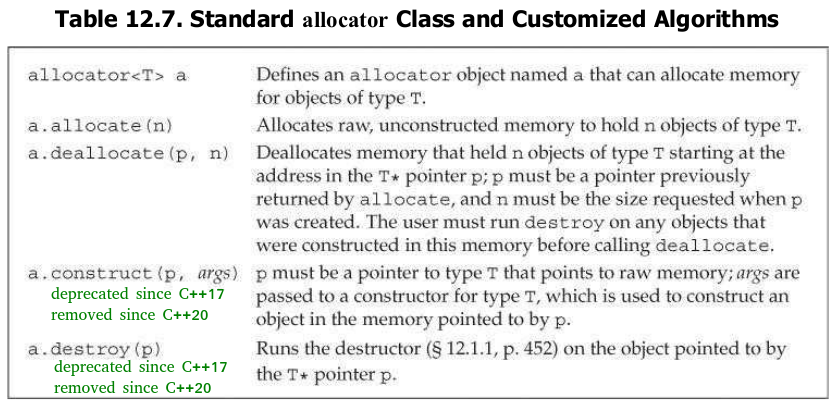
\includegraphics[width=\textwidth]{figures/allocator_operations.png}
    \end{center}
\end{frame}

\begin{frame}[fragile]{Allocators}
    \ttt{std::vector<T>} uses \ttt{std::allocator<T>} by default.
    \begin{cpp}
std::vector<int> v1;
std::vector<int, std::allocator<int>> v2;
std::vector<int, gkxx::Simple_allocator<int>> v3;
    \end{cpp}
\end{frame}